\documentclass{journal}

\title{Deep Learning: A Survey}
\author{Nathaniel Beckemeyer}

% Some packages that I use in every document
\usepackage{comment}
\usepackage{microtype}
\usepackage{booktabs}
\usepackage[utf8]{inputenc}
\usepackage{hyperref}
\usepackage{lmodern}
\usepackage[obeyDraft]{todonotes}

% This document
\usepackage{amsmath}
\usepackage{graphicx}
\graphicspath{{Figures/}}


\begin{document}

\maketitle{}

\section{Introduction}
My initial ideas were to attept to classify the CIFAR-10 image
dataset using a convolutional neural network (CNN) and autoendcoding
the MNIST dataset. When I searched for how to get started, both of these tasks
had already been implemented---the CIFAR-10 task was actually a TensorFlow
tutorial already! So instead, in order to gain intuition for the types of
problems that deep learning is able to solve, I opted to try to use deep
learning on a variety of
tasks rather than try to do something in-depth with a
CNN or some other deep neural network.

Rather than write all of my
own code from scratch, I mostly used the TensorFlow code that others had already
written to experiment with 5 tasks:
\begin{enumerate}
    \item{Classifying the CIFAR-10 dataset\footnote{Alex Krizhevsky:
          \url{https://www.cs.toronto.edu/~kriz/cifar.html}} with a CNN.}
    \item{Using a recurrent neural network (RNN) to predict words in the
          Penn Tree Bank (PTB)\footnote{Tomas Mikolov:
          \url{http://www.fit.vutbr.cz/~imikolov/rnnlm/simple-examples.tgz}}
          dataset.}
    \item{Using a wide and deep network to classify adults as having income
          greater than or less than \$50000.\footnote{UCI
          Machine Learning Repository:
          \url{https://archive.ics.uci.edu/ml/datasets/adult}}}
    \item{Using the `word2vec' method to approximate semantic distance
          between words.\footnote{Matt Mahoney:
          \url{http://mattmahoney.net/dc/text8.zip}}}
    \item{Using an autoencoder to encode MNIST digits.\footnote{Ships with
          TensorFlow}}
\end{enumerate}

The remainder of the report will be composed of descriptions of the experiments,
their results, and brief discussions of each.


\section{Experiments}
\subsection{CNN on the CIFAR-10 dataset}
This task was fairly straightforward: Image classification. Given 60000 labeled
32x32 images, the goal was to classify new images into 10 categories: Airplane,
automobile, bird, cat, deer, dog, frog, horse, ship, and truck.

Because we've covered CNNs in class, I won't go into detail on how they work; it
suffices to provide the pipeline of this network:
Inputs go through two iterations of a convolutional layer, a norm response
layer, and max pooling; then, through two ReLU layers to a linear
softmax (for generating logits) output layer.

I followed the TensorFlow tutorial
to do this part; in the code that they provide, however, the CNN training
runs over the course of 1000000 steps, but I only ran it for 2000 in order
to expedite termination. Despite such a few number of steps, it
classified images with 65.7\% accuracy (where accuracy is defined as
output where the highest likelihood class is the correct class).

\subsection{RNN on the PTB dataset}
\subsubsection{RNNs}
Next, I wanted to use a recurrent neural network to predict words in a
sequential reasoning task.

The recurrent neural network were what I learned is called \emph{Long Short
Term Memory Networks,} (LSTMs) which is a special kind of RNN for remembering
state for long periods of time. See Figure~\ref{fig:LSTM} for a visualization
of the network\footnote{This image, along with my understanding of LSTMs, comes
from Christopher Olah's blog at
\url{http://colah.github.io/posts/2015-08-Understanding-LSTMs/}},
which I will explain briefly. It helps me to think of the top line as the
\emph{state line} and the bottom one as the \emph{observation line}, which
is a combination of the previous output and the current inputs.
%
\begin{figure}[h]
    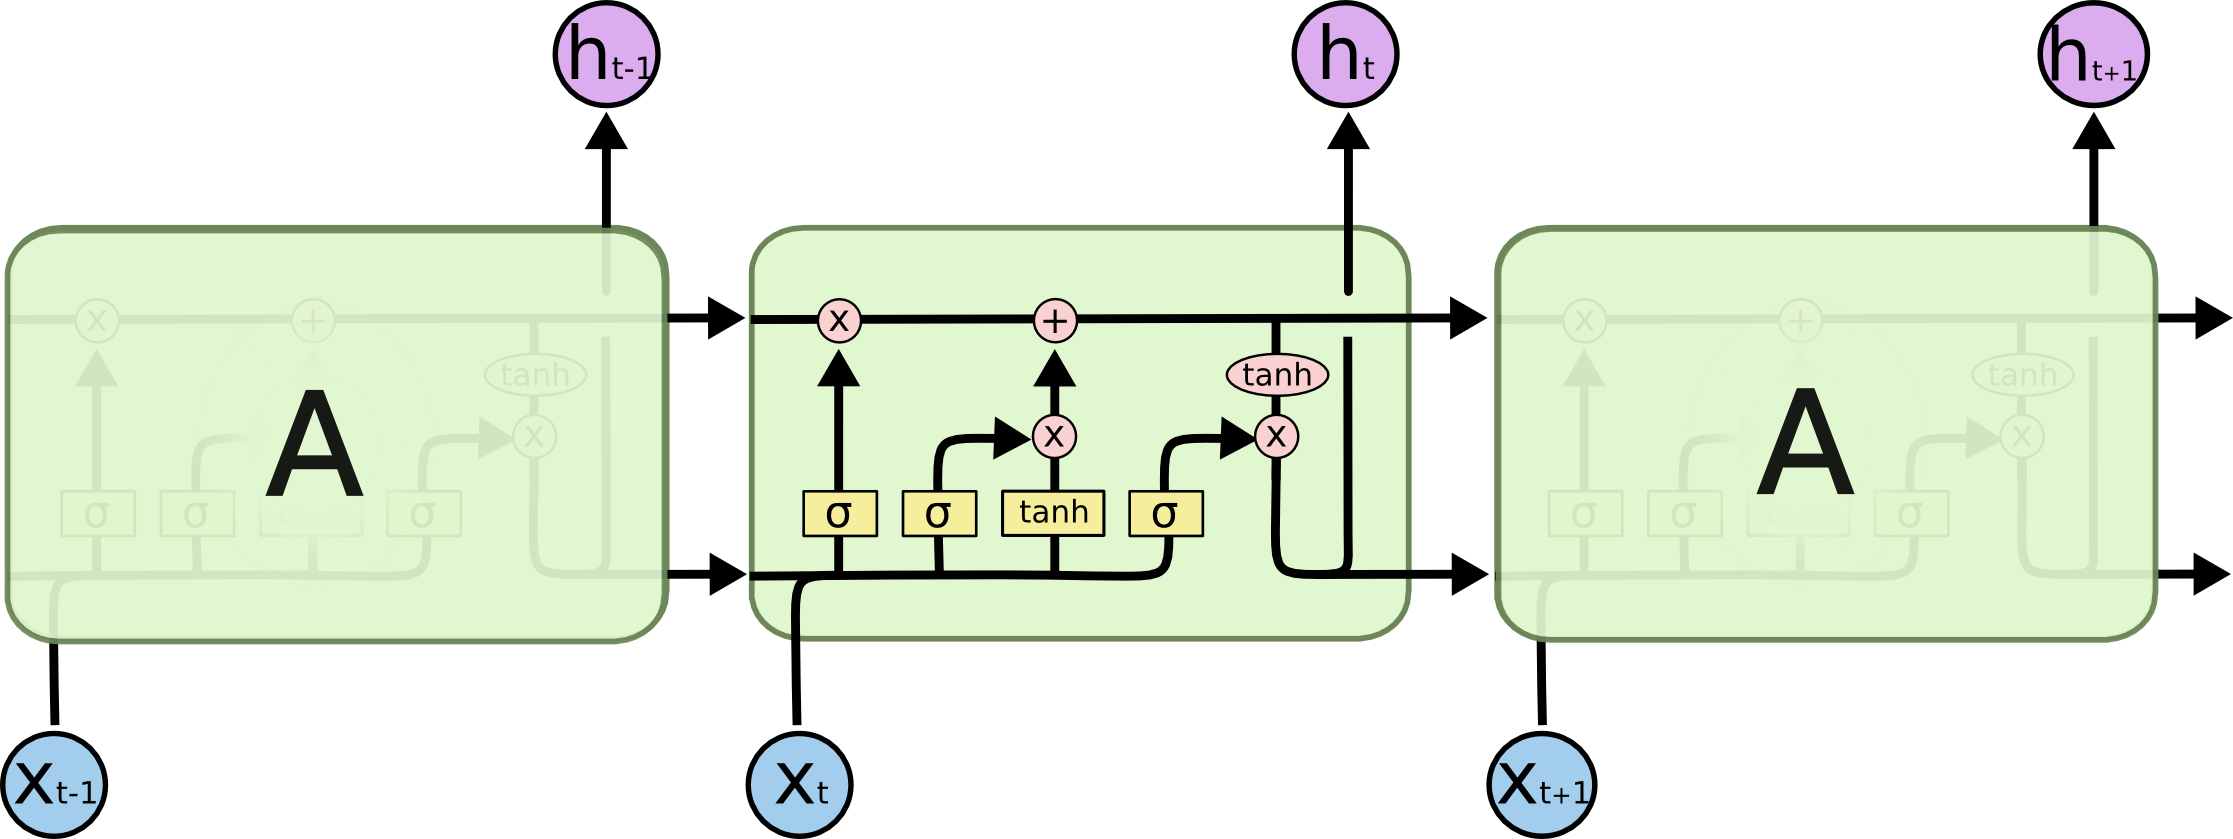
\includegraphics[width=\textwidth]{LSTM}
    \caption{A visualization of an unrolled LSTM RNN.}\label{fig:LSTM}
\end{figure}
%
The LSTM network consists of four special layers of artificial neurons---they
are special because they are not merely sequential layers, but rather they
interact differently.

The leftmost layer in the diagram above is the \emph{forget gate,}
and it identifies which features from the observation line should not be
included in the new state. The state line is multiplied by the output
from this layer to forget the unimportant features of the output.

The layer to its right is called the \emph{input gate}. It identifies
which features from the observation line are important to store in the current
state. This gate interacts with the \emph{candidate values}, generated by
the $\tanh{}$ layer. These two outputs are multiplied to select the changes in
important features, and added to the state line to represent the current state.

The final layer is the \emph{output gate}. It helps select the features from
the observation line that are important; these features are then multiplied by
the state line (scaled by $\tanh{}$ to be between -1 and 1) to generate the new
output. (The reason for naming the sigmoidal layers the gates is to scale the
values to be between 0 and 1, which is good for measuring relative importance.)

\subsubsection{Task}
The RNN task is to predict next words in the PTB dataset. First, the words
are embedded into a dense representation. Then, the LSTM does repeated batch
gradient descent on a series of words. The loss function for a series of
examples follows.
$$L \leftarrow{} {-\frac{1}{N}\sum\limits_{i=1}\limits^{N}\ln{p_{target}}}$$
This is the natural logarithm of the average per-word perplexity, which is the
result reported for this task (and, according to the tutorial I was looking at,
typical of NLP tasks in general---we used perplexity of n-gram models in
the advanced AI course): I ran code on this dataset for 13 epochs
(or complete runthroughs of the test set), and, ultimately, it achieved a test
perplexity score of 115.3.

Unfortunately, I don't have a good grasp of what that number means;
reverse-engineering the formula for perplexity implies that the
average logarithm probability is -4.75, or the average probability is $0.8\%$.
That's more useful, but I don't have a good baseline for comparison.

Ultimately, I think that this task was the most fascinating of all of the ones
that I did, and perhaps because I understand it least. For instance, it is
unclear to me why the input gate and candidate values could not be merged into
a single $\tanh{}$ layer that polarizes on important values and approaches 0 on
unimportant values. I suspect that it has to do with the mathematics of the
backpropogation. I plan to explore this area much more in the future.

\subsection{Wide \& Deep Learning}
This task comprised of predicting whether an individual earned more or less
than \$50000 based on their corresponding census data. Intriguingly, it
focused on combining a `wide' learning model with a deep learning one. See
Figure~\ref{fig:WideDeep} for a visualization.\footnote{This visualization,
and the task, come from the corresponding TensorFlow tutorial:
\url{https://www.tensorflow.org/tutorials/wide_and_deep}.}
The purpose of the wide model is to memorize interactions between many sparse
features, such as the combination of age, education, and native country. For
continuous features, or features with very many values, buckets (akin to tiling
in reinforcement learning in continuous domains) or hashing were performed.

\begin{figure}[h]
    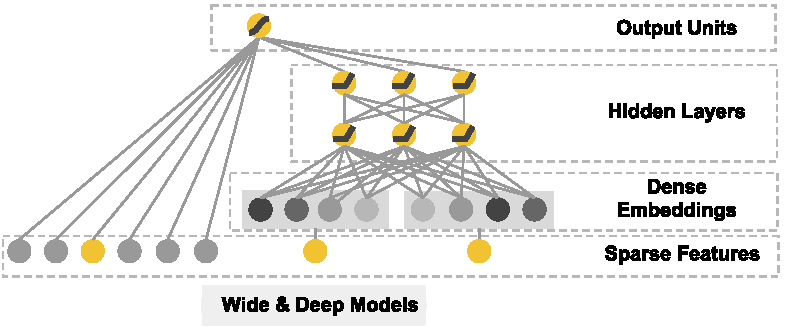
\includegraphics[width=\textwidth]{wide_n_deep}
    \caption{A wide \& deep neural network example.}\label{fig:WideDeep}
\end{figure}

The end classifier is a linear classifier that combines input from all of the
wide columns the last layer from the deep neural network (which had two hidden
layers with 200 and 100 nodes each). I tried to play around with the size of
the networks and the sparse feature columns (i.e., adding more for the
combination of multiple input features), but I never managed to get the accuracy
above 85\%, which was only slightly (and probably not significantly) above the
baseline accuracy of the tutorial.

I had never thought of using very many columns to represent interactions between
different features and memorize results before---that was an incredibly neat
trick. It also made me wonder about the performance of other types of
bucketizations; things like Gaussian distances, rather than buckets, for
instance.

\subsection{word2vec}
This task was simply an experiment to try to understand how the word2vec
algorithm worked. The principle idea behind this algorithm is to vectorize
words to prevent sparsity by assuming that words that appear close to each
other are semantically similar, and guessing at different dimensions of
meaning. These dimensions are called \emph{embeddings}.

These embeddings are calculated as the hidden layer of a neural network. In
this case, the input to the network is a word, and the output from the network
is the context from that word; in other words, the network tries to predict
the surrounding words from a given word!

I ran this model using a vocabulary of the 50000 most common (anything
else was replaced with an unknown tag) words from the
dataset mentioned above, following a tutorial on the
TensorFlow website. The number of contextual words was
2---one on each side of the target word (the predictor). There were
128 embeddings. The 1000 most common words were projected from the 128
dimensions the algorithm selected into two dimensions using a technique
called \emph{t-Distributed Stochastic Neighbor Embedding} (tSNE). tSNE
defines a probability distribution where numbers that are close to each other
in the high dimensional space have high probability, and does the same thing
for numbers in the low-dimensional space. It then minimizes the Kullback-Leibler
divergence of the high-dimensional distribution from the low-dimensional
distribution, using gradient descent to assign the parameters of the
low-dimensional one. The result is visualized in Figure~\ref{fig:tsne}

\begin{figure}[h]
    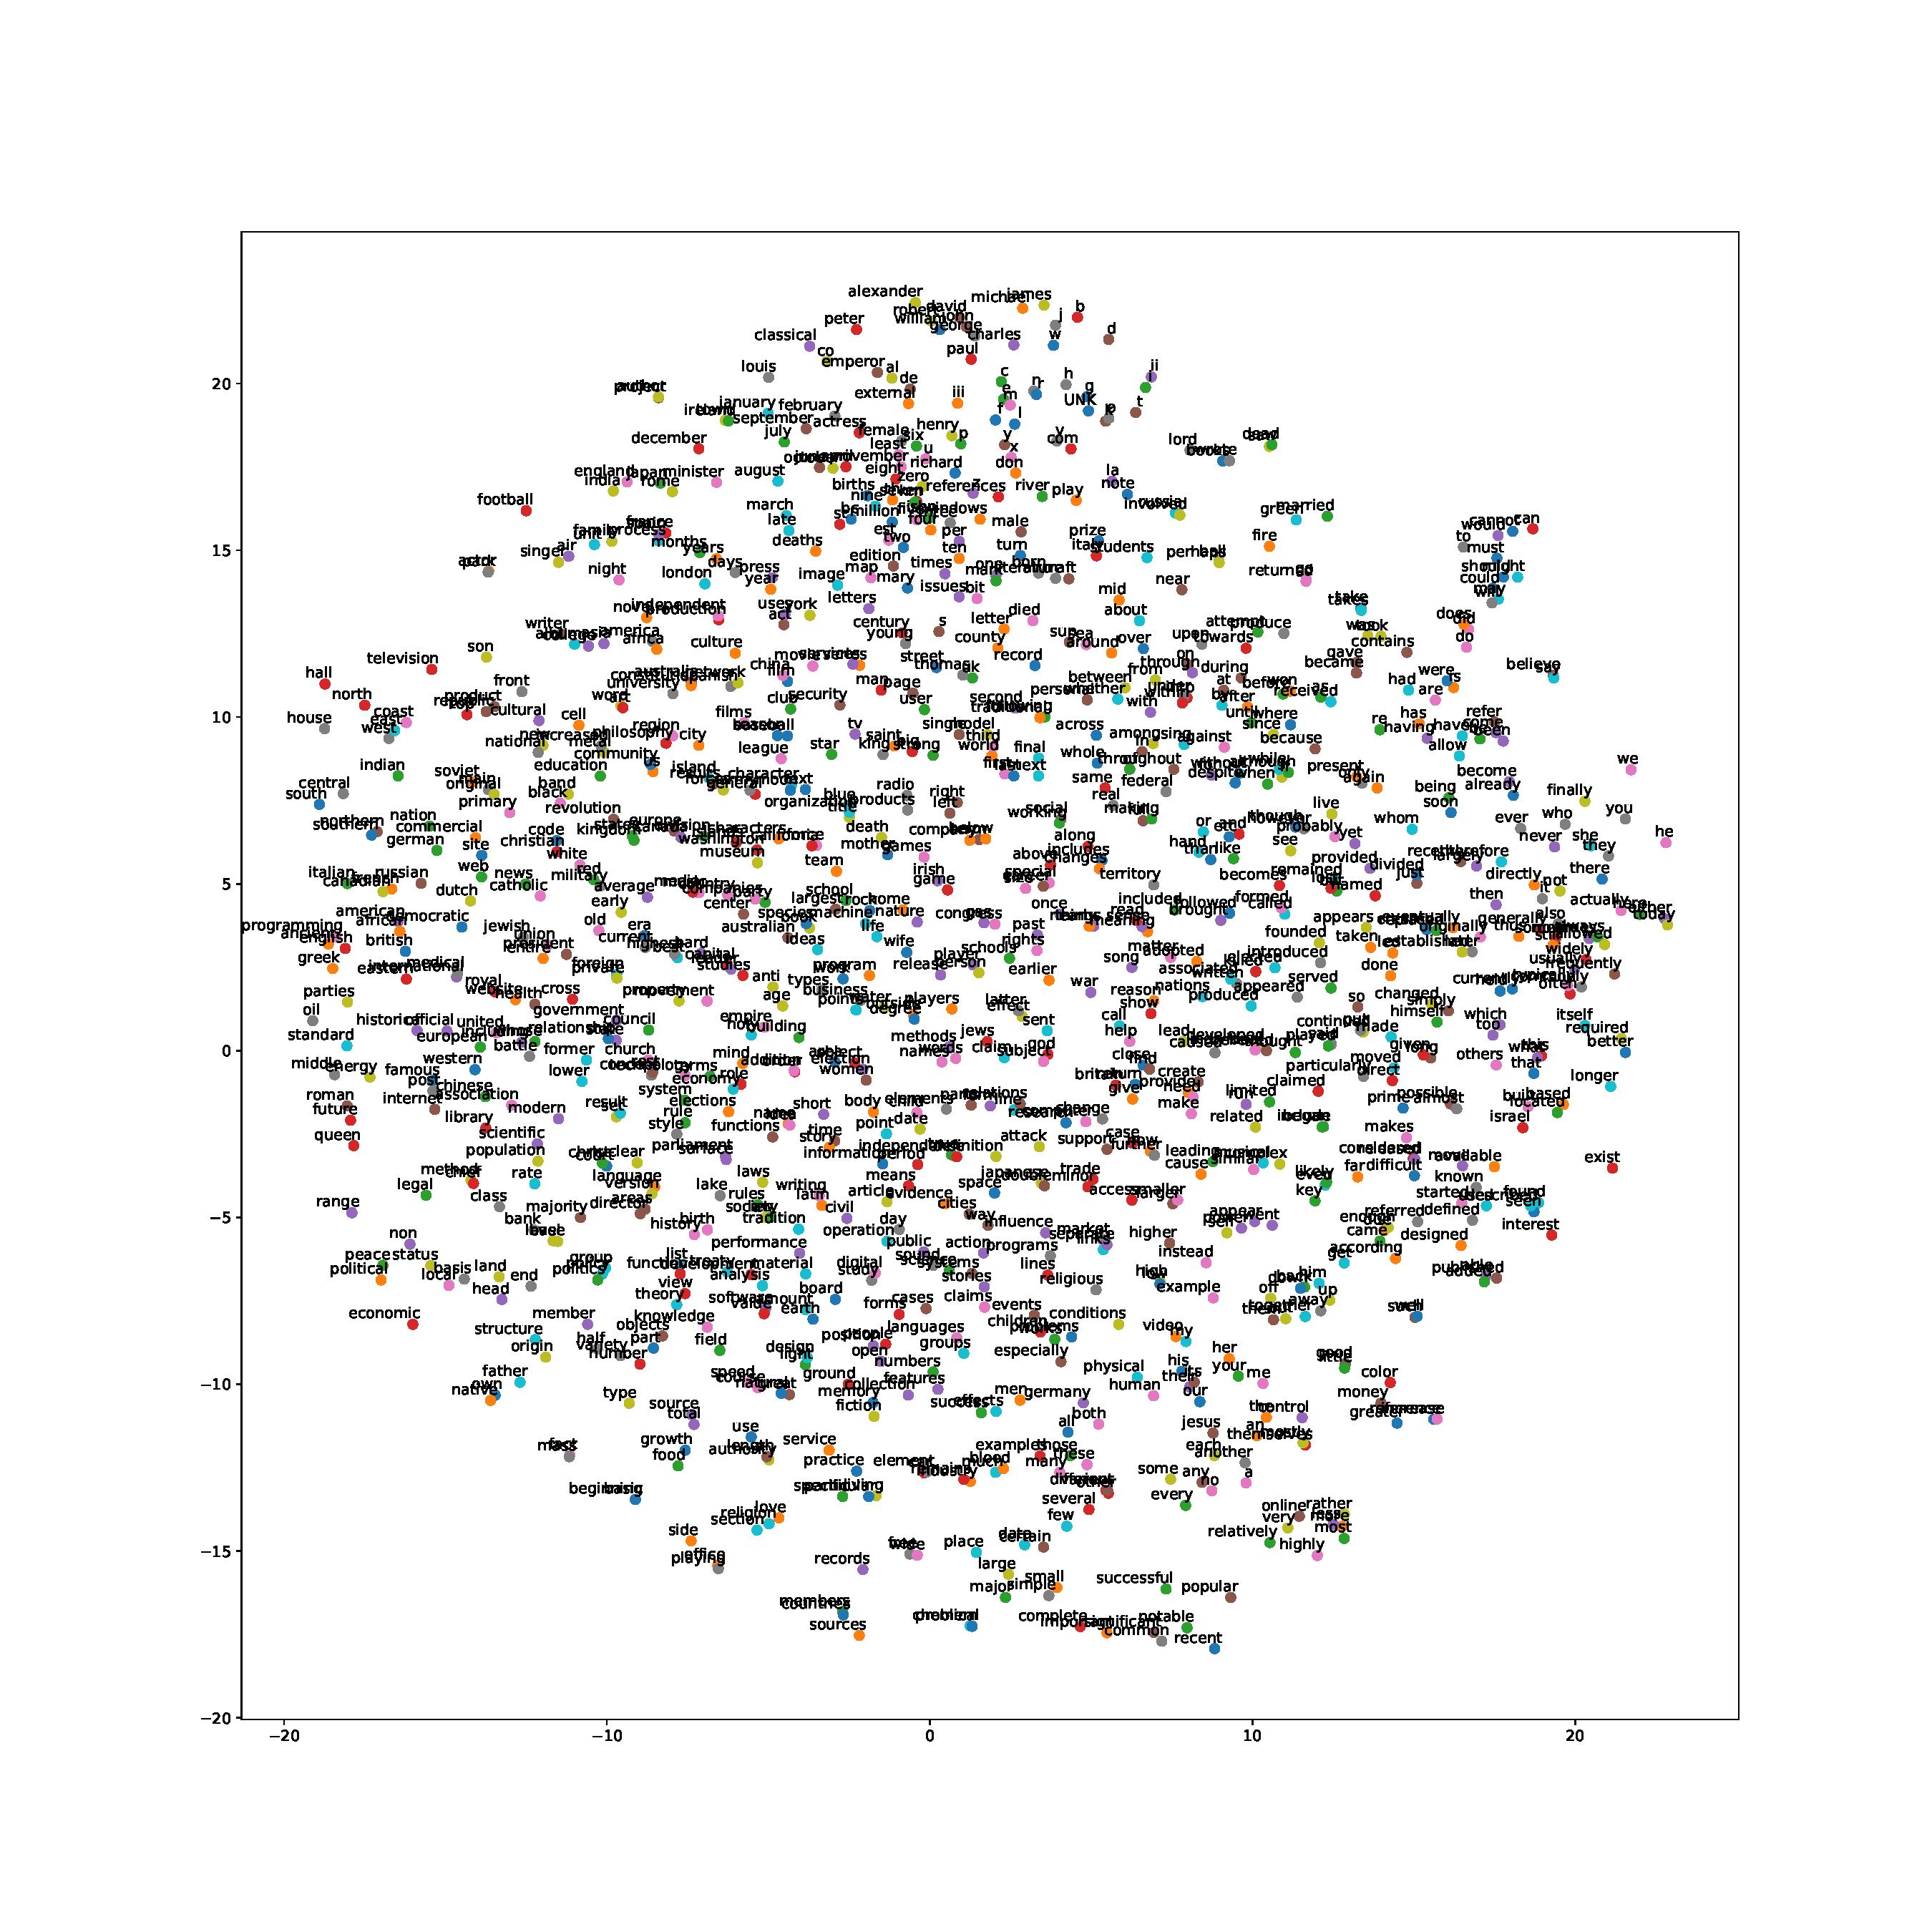
\includegraphics[width=\textwidth]{tsne}
    \caption{A wide \& deep neural network example.}\label{fig:tsne}
\end{figure}

In the future, I would like to try this on a more domain-specific dataset, and
see how well it distinguishes the various concepts within that domain. I expect
that it will do well, as only the relative usage of words matters.

\subsection{MNIST Autoencoding}
This last task was very simple. When I searched for autoencoding MNIST, the top
result was code doing just that. It's a very simple neural network, and I played
with it slightly to try to change the results (and modified it to visualize the
encodings). There were three hidden layers: A 256-unit layer, a 144-unit layer,
and then another 256-unit layer.

Autoencoding is a technique for encoding data in neural networks where the
network is trained to make its output match its input exactly; the secret lies
in the front half of the network where the data is encoded. By cutting the
network into two, where the center layer is the output the first network and
the input of the second network, you get encoding and decoding networks,
respectively.

The results of this exercise are visualized in Figure~\ref{fig:autoencoding}.

\begin{figure}[h]
    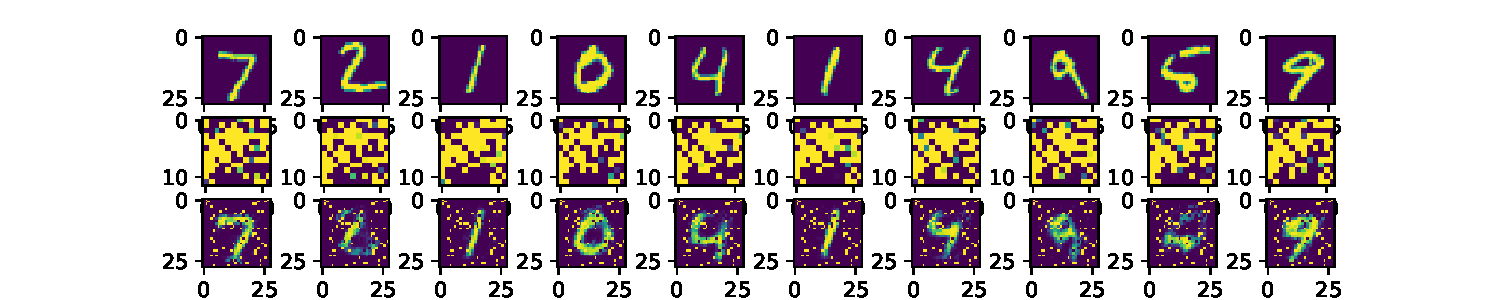
\includegraphics[width=\textwidth]{MNIST_Autoencoding}
    \caption{The MNIST autoencoding visualization. The top layer is the 28x28
             original MNIST data. The middle layer is the 12x12 encoded version,
             and the output layer is the 28x28
             reconstruction.}\label{fig:autoencoding}
\end{figure}

\end{document}
